\subsection{Register Directory}
\begin{figure}[H]
	\centering
	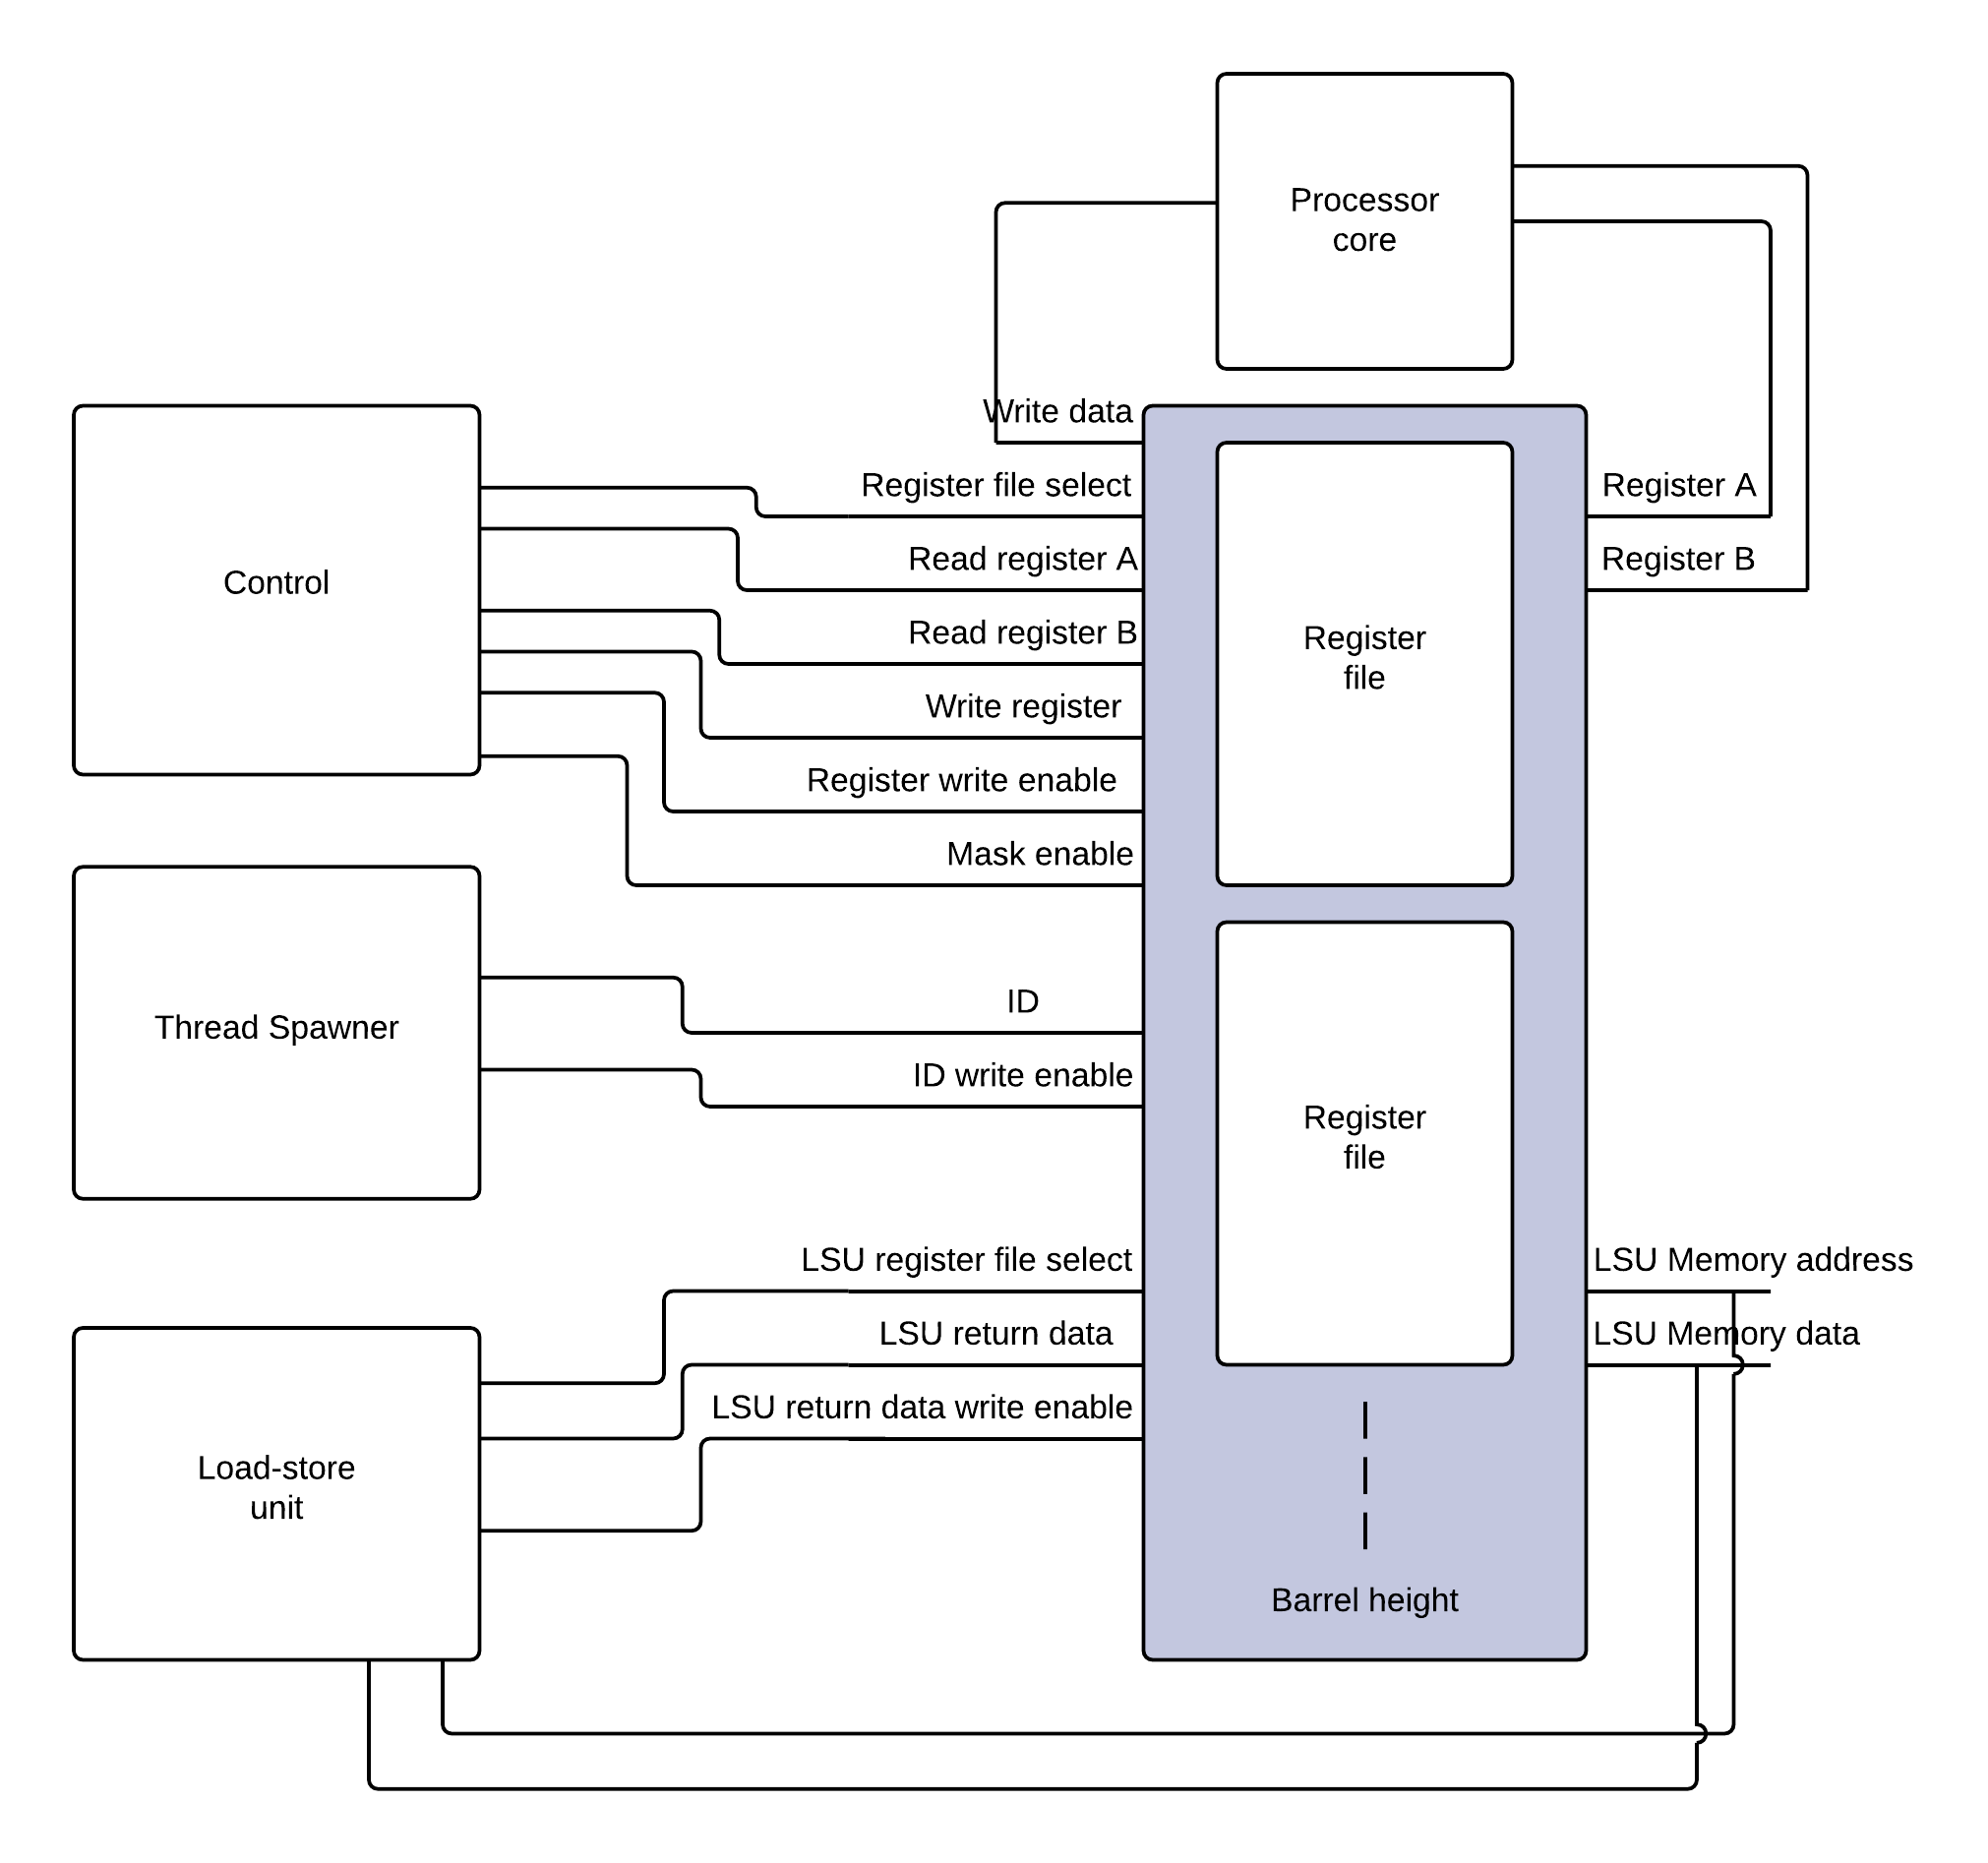
\includegraphics[width=\textwidth]{../gpu/diagrams/register_directory.png}
	\caption{The register directory, and its neighboring components.}
	\label{fig:register_directory}
\end{figure}

There is one register directory per processor core.
Each register directory contains one register file per barrel line.
The register files include seven dedicated registers, and nine general purpose registers, listed in table \ref{tab:registers_overview}.

\begin{table}[H]
	\centering
	\begin{tabular}{|c|c|c|}
		\hline Register number & Description & RW \\ 
		\hline \$0 & Zero register & Read-only \\ 
		\hline \$1 & ID High & Read/Write \\ 
		\hline \$2 & ID Low & Read/Write \\ 
		\hline \$3 & Address High & Read/Write \\ 
		\hline \$4 & Address Low & Read/Write \\ 
		\hline \$5 & LSU data & Read/Write \\ 
		\hline \$6 & Masking register & Write \\ 
		\hline \$7 - \$15 & General purpose registers & Read/Write \\ 
		\hline 
	\end{tabular} 
	\caption{The registers contained within the register files.}
	\label{tab:registers_overview}
\end{table}

Individual register files are selected by using the \emph{register file select} signal.
Using this signal, the warp scheduler selects the active register file.
Within the register directory, signals are routed to the active register file using the select signal.
Consequently, from the processor core's point of view, there's just one register file.

In the architecture the dedicated registers have special functions.
<direct access>
Ignoring registers \$0 and \$6, the dedicated registers may be used as general purpose registers.


The masking register is used to enable conditional execution.
When executing predicated instructions, the masking register is used to disable writes to the register file.
This makes the instruction have no effect (Figure \ref{fig:masking}).
To reduce the complexity of the architecture \emph{store word} instructions cannot be predicated.
Instead the programmer has to manage the values written explicitly.
\begin{figure}[H]
	\centering
	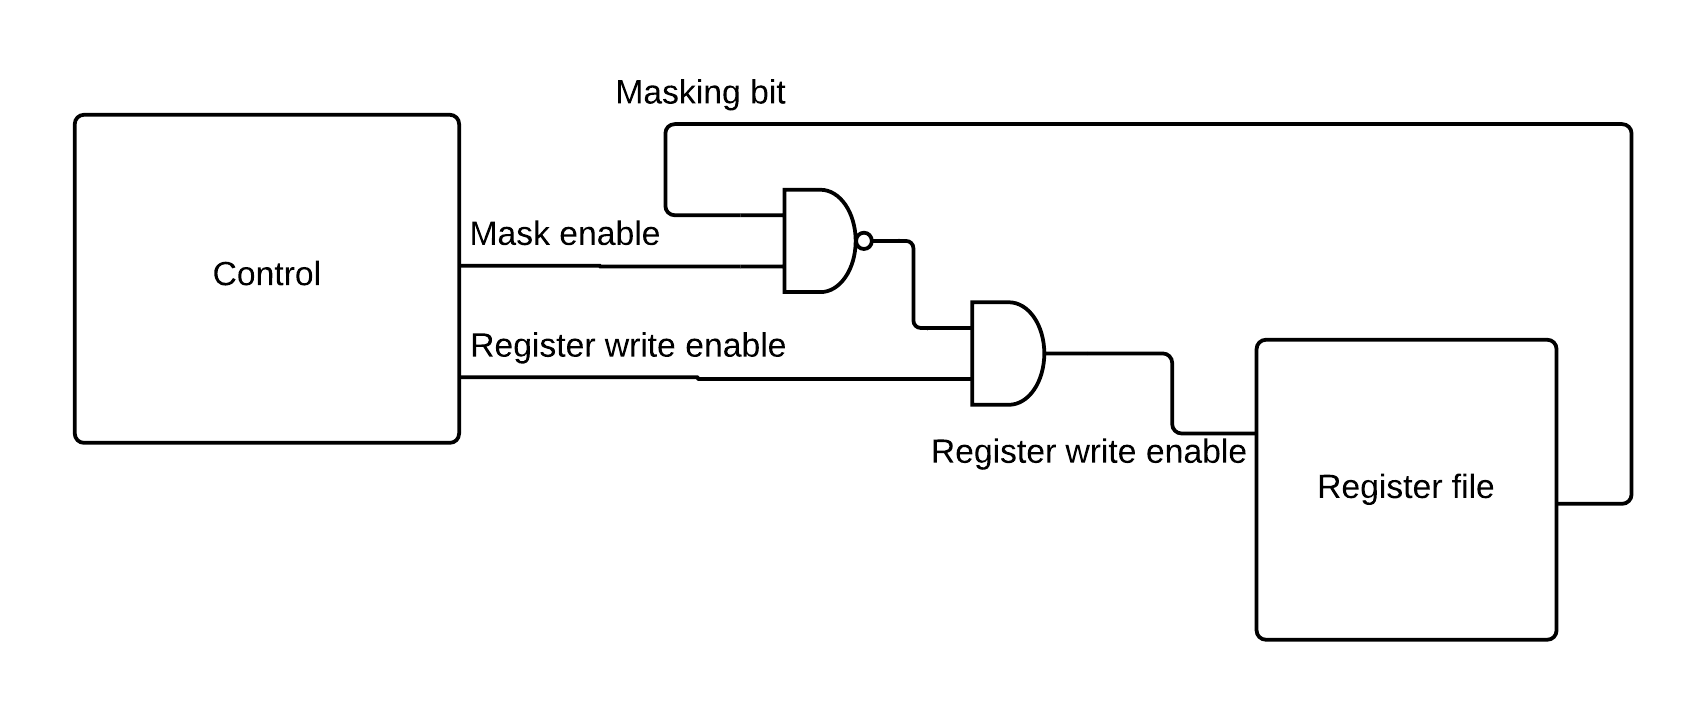
\includegraphics[width=0.8\textwidth]{../gpu/diagrams/masking.png}
	\caption{Using the mask bit to disable register writes.}
	\label{fig:masking}
\end{figure}

Data memory addresses are 20 bit wide, and thread IDs are 19 bit wide.
The word size is only 16 bits.
To represent these values they are split into two registers which contain the higher and lower bits.

The load store unit (LSU) has a separate signal for selecting which register file to write to.
Using this signal, the LSU can write data loaded from memory into any register files on its own.
